\documentclass[a4paper,10pt]{article}
\usepackage[utf8]{inputenc}
\usepackage[spanish]{babel}
\usepackage{fancyhdr}
\usepackage{multicol}
\usepackage{geometry}
\usepackage{graphicx}
\usepackage{float}  
\usepackage{amsmath}
\usepackage{listings}
\usepackage[utf8]{inputenc}
\usepackage{xcolor}
\geometry{a4paper, portrait, margin=1in}
\lstset{
  language=Python,
  basicstyle=\ttfamily\small,
  breaklines=true,
  frame=single,
  showstringspaces=false
}

\pagestyle{fancy}
\fancyhf{}
\fancyhead[L]{\textbf{Métodos de Optimización}}
\fancyhead[R]{Universidad Nacional del Altiplano - FINESI}
\fancyfoot[C]{\thepage}


\begin{document}
\begin{titlepage}
    \centering
    \vspace*{4cm}

    {\LARGE \textbf{UNIVERSIDAD NACIONAL DEL ALTIPLANO}}\\[0.5cm]
    {\Large \textbf{Escuela Profesional de Ingeniería Estadística e Informatica}}\\[3cm]

    {\huge \textbf{Método de Gauss-Jordan}}\\[2cm]

    \textbf{Integrantes:}\\
    Lizbeth Estefany Caceres Tacora\\
    Ronaldo Carlos Mamani Mena\\
    Carlos Paolo Fontanil Barrera\\[2cm]

    \textbf{Puno - Perú}\\
    \textbf{2025}
\end{titlepage}
\section{Introducción}
El método de eliminación de Gauss-Jordan es una variante del método de Gauss. La diferencia principal es que, en lugar de resolver el sistema con sustitución hacia atrás, lleva la matriz aumentada a una forma escalonada reducida por filas mediante operaciones elementales. Esta mejora fue propuesta por el ingeniero alemán Wilhelm Jordan. Mientras que el método de Gauss obtiene el sistema equivalente en forma escalonada, el método de Gauss-Jordan lo lleva un paso más allá, simplificando aún más la matriz para obtener directamente la solución del sistema.

\section{Solución de sistemas de ecuaciones lineales mediante el método de reducción de Gauss-Jordan}
En esta parte el lector hallará la solución de sistemas de ecuaciones lineales usando el Método de Gauss-Jordan. El tema se presenta en cuatro secciones: 
\begin{itemize}
    \item A) Sistemas con solución única
    \item B) Sistemas con infinidad de soluciones
    \item C) Sistemas sin solución
    \item D) Sistemas homogéneos
\end{itemize}

\begin{figure}[H]
    \centering
    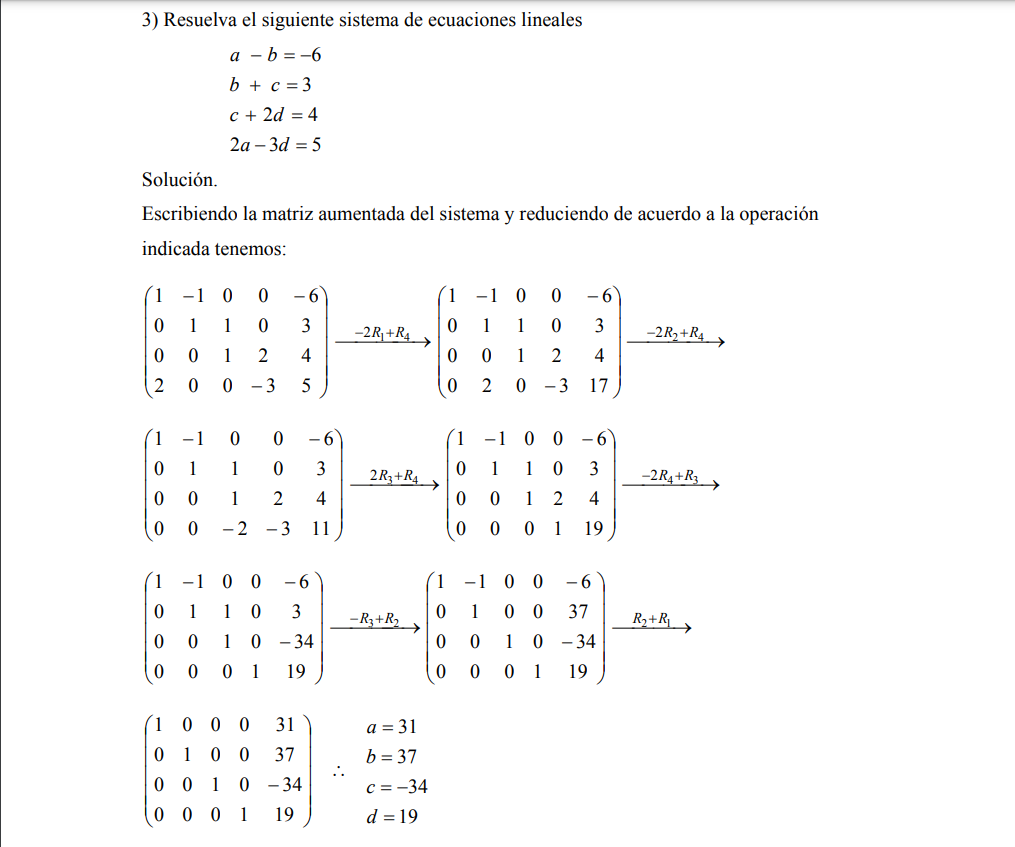
\includegraphics[width=1\linewidth]{image.png}
    \caption{A) Sistema con solución única}
\end{figure}
\vspace{2em}
\begin{figure}[H]
    \centering
    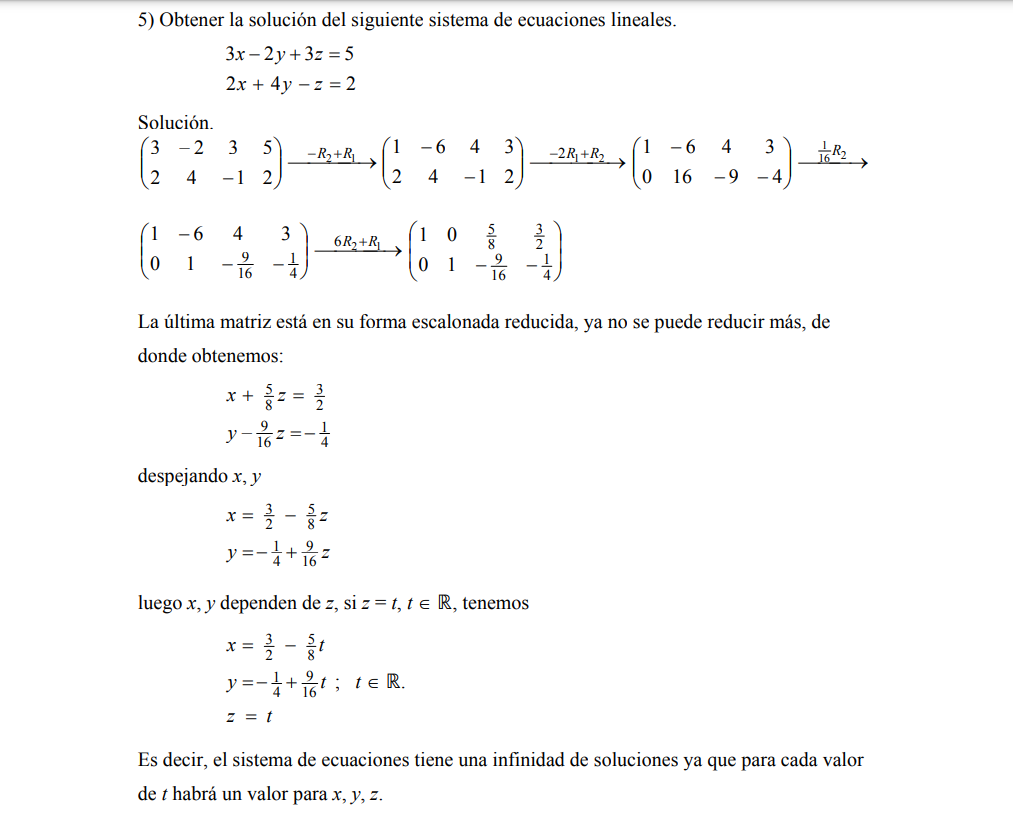
\includegraphics[width=1\linewidth]{2.png}
    \caption{B) Sistema con infinidad de soluciones}
\end{figure}
\vspace{4em}
\begin{figure}[H]
    \centering
    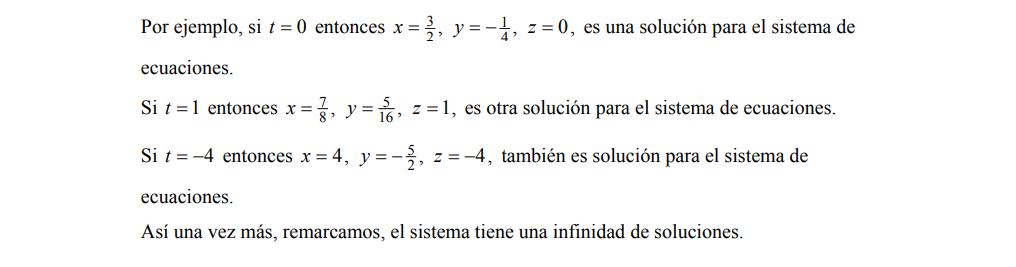
\includegraphics[width=1\linewidth]{3.png}
    \caption{Ejemplo intermedio del proceso de reducción}
\end{figure}

\begin{figure}[H]
    \centering
    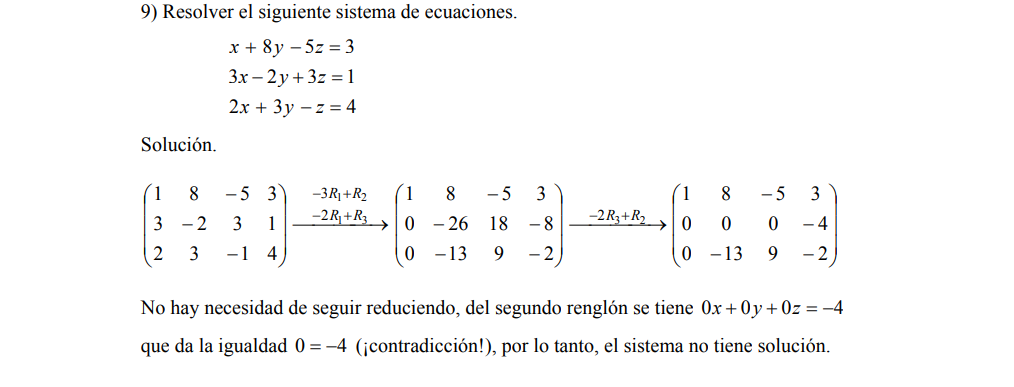
\includegraphics[width=1\linewidth]{4.png}
    \caption{C) Sistema sin solución}
\end{figure}
\vspace{6em}
\begin{figure}[H]
    \centering
    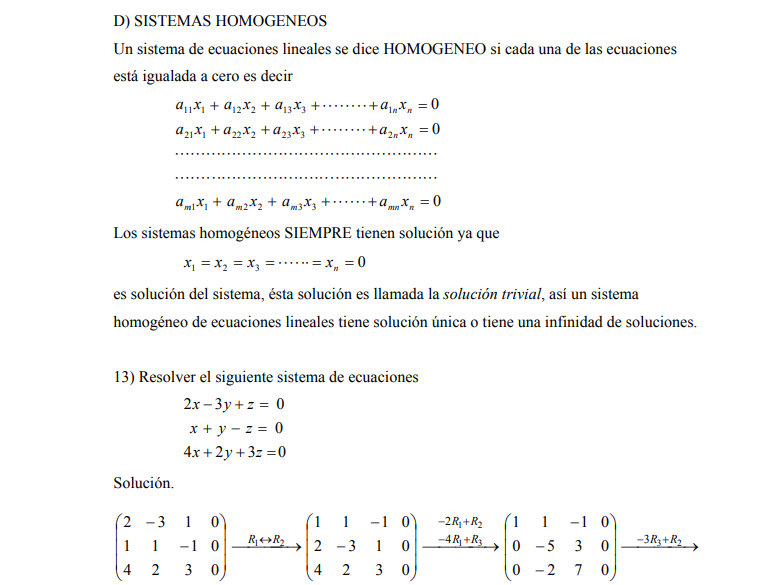
\includegraphics[width=1\linewidth]{5.png}
    \caption{D) Sistema homogéneo}
\end{figure}

\begin{figure}[H]
    \centering
    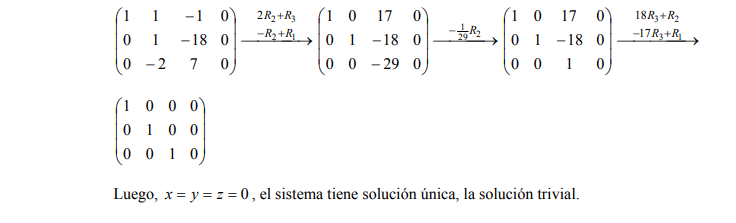
\includegraphics[width=1\linewidth]{6.png}
    \caption{E) Sistema homogéneo}
\end{figure}



\section{Utilizando el método de Gauss-Jordan en la función de presión arterial}

Para ilustrar cómo se utiliza el \textbf{Método de Gauss-Jordan} para resolver un sistema de ecuaciones con las incógnitas \textbf{pulsaciones} (\(P\)) y \textbf{tiempo de actividad física} (\(T\)), consideramos el siguiente sistema de ecuaciones, que modela la relación entre la presión arterial, las pulsaciones y el tiempo de actividad física.



\subsection{Sistema de Ecuaciones}

El sistema de ecuaciones que modela la relación entre las variables es el siguiente:





\[
2P + T = 340
\]

\[
3P - T = 450
\]

Donde:

- \( P \): pulsaciones por minuto.

- \( T \): tiempo de actividad física en minutos.
\vspace{1em}

Aunque en la realidad, la relación entre las pulsaciones y el tiempo de actividad física con respecto a la presión arterial no es lineal, para fines prácticos y de simplificación, podemos aproximar la relación mediante funciones lineales.

\vspace{2em}
\textbf {Estas incógnitas tienen restricciones, tales como:} 

Las pulsaciones (\(P\)) tienen un rango delimitado que va desde 100 hasta 190 pulsaciones por minuto, ya que, según la especialista, el rango de pulsaciones adecuadas varía dependiendo de la condición física y la edad de la persona.

El tiempo de actividad física (\(T\)) está delimitado entre 20 minutos y 180 minutos, ya que, según las recomendaciones de la OMS, el tiempo de actividad física saludable debe estar dentro de este rango.

\vspace{1em}
\begin{figure}[H]
    \centering
    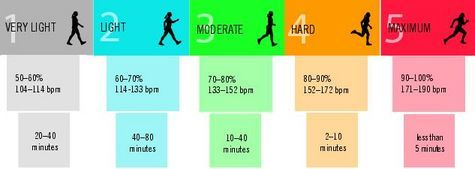
\includegraphics[width=0.75\textwidth]{1366_2000.jpg}
    \caption{La frecuencia cardíaca y el entrenamiento ¿cómo se calcula, qué valores son adecuados?.}
    \label{fig:presion}
\end{figure}
\textit{Fuente: Vitónica, 2008}
\vspace{2em}

De la misma forma en cuanto a los posibles valores que pueden llegar a darase para la presion arterial con respecto a estas dos variables tenemos el siguiente cuadro:

\vspace{1em}
\begin{figure}[H]
    \centering
    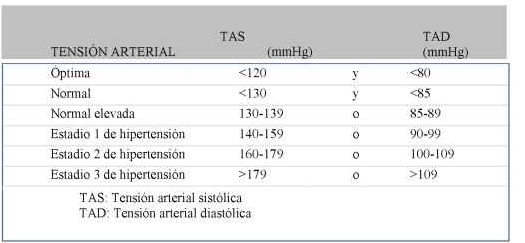
\includegraphics[width=0.6\textwidth]{clasificacion_jnc.png}
    \caption{Clasificación de la hipertensión arterial según el JNC 1997.}
    \label{fig:jnc1997}
\end{figure}
\textit{Fuente: Report of the Joint National Committee, 1977}
\vspace{2em}

\section*{Paso 1: Representación Matricial}

El sistema de ecuaciones se representa en forma aumentada como:

\[
\begin{bmatrix}
2 & 1 & | & 340 \\
3 & -1 & | & 450
\end{bmatrix}
\]

\section*{Paso 2: Hacer que el Primer Pivote Sea 1}

Dividimos la primera fila entre \(2\):

\[
\text{Fila 1} = \frac{1}{2} \times \text{Fila 1}
\]

Resultado:

\[
\begin{bmatrix}
1 & 0.5 & | & 170 \\
3 & -1 & | & 450
\end{bmatrix}
\]

\section*{Paso 3: Eliminar el Primer Elemento de la Segunda Fila}

Restamos \(3 \times\) la primera fila de la segunda fila:

\[
\text{Fila 2} = \text{Fila 2} - 3 \times \text{Fila 1}
\]

Resultado:

\[
\begin{bmatrix}
1 & 0.5 & | & 170 \\
0 & -2.5 & | & -60
\end{bmatrix}
\]

\section*{Paso 4: Hacer que el Segundo Pivote Sea 1}

Dividimos la segunda fila entre \(-2.5\):

\[
\text{Fila 2} = \frac{1}{-2.5} \times \text{Fila 2}
\]

Resultado:

\[
\begin{bmatrix}
1 & 0.5 & | & 170 \\
0 & 1 & | & 24
\end{bmatrix}
\]

\section*{Paso 5: Eliminar el Segundo Valor de la Primera Fila}

Restamos \(0.5 \times\) la segunda fila de la primera fila:

\[
\text{Fila 1} = \text{Fila 1} - 0.5 \times \text{Fila 2}
\]

Resultado:

\[
\begin{bmatrix}
1 & 0 & | & 158 \\
0 & 1 & | & 24
\end{bmatrix}
\]

\subsection{Solución Final}

Las soluciones para las incógnitas \(x_1\) y \(x_2\) son:

\[
x_1 = 158 \quad \text{y} \quad x_2 = 24
\]

\subsection{Interpretación de los Resultados}

\subsection*{Variable \(x_1\)}

- \textbf{Valor de } \( x_1 = 158 \). Este valor podría interpretarse como una cantidad importante dependiendo del contexto (por ejemplo, pulsaciones, calorías, o alguna medida relevante en el problema). 

\subsection*{Variable \(x_2\)}

- \textbf{Valor de } \( x_2 = 24 \). Este valor puede representar una cantidad de minutos, unidades, o una variable relacionada con la actividad física u otra métrica según el contexto.

\subsection*{Análisis del Valor \(x_2 = 24\) minutos}

\textbf{Rango saludable:} Según la OMS, el tiempo recomendado de actividad física para adultos está entre \textbf{20 y 180 minutos} diarios.

\textbf{Interpretación:}
\begin{itemize}
    \item El valor obtenido ($x_2 = 24$ minutos) está \textbf{dentro del rango recomendado}.
    \item Este tiempo puede corresponder a una sesión corta de actividad física moderada, como una caminata rápida.
    \item Se considera un mínimo saludable, aunque podrían recomendarse sesiones más largas para mayores beneficios.
\end{itemize}

\subsection*{Relación entre \(x_1\) y \(x_2\)}

Aunque el modelo es una simplificación lineal, los valores obtenidos:
\begin{itemize}
    \item Satisfacen el sistema original de ecuaciones planteado:  
    \[
    \begin{cases}
    2x_1 + x_2 = 340 \\
    3x_1 - x_2 = 450
    \end{cases}
    \]
    \item Pueden representar una relación proporcional entre dos variables relacionadas con salud, economía o rendimiento físico, dependiendo del caso.
\end{itemize}

\subsection*{Limitaciones del modelo}
\begin{itemize}
    \item \textbf{Simplicidad:} El sistema de ecuaciones asume una relación lineal entre variables, lo que no siempre representa la realidad.
    \item \textbf{Falta de contexto:} No se proporciona el significado específico de \(x_1\) y \(x_2\), lo que limita la interpretación precisa.
    \item \textbf{Factores externos:} No se consideran otros factores importantes como edad, estado físico, condiciones médicas, etc.
\end{itemize}

\subsection{Código Python en texto plano}
\begin{verbatim}
def gj(m):
 n=len(m)
 for j in range(n):
  if m[j][j]==0:
   try:m[j],m[next(i for i in range(j+1,n)if m[i][j]!=0)]=m[next(i for i in range(j+1,n)if m[i][j]!=0)],m[j]
   except:raise ValueError("No solución única")
  m[j]=[x/m[j][j]for x in m[j]]
  for i in range(n):
   if i!=j:m[i]=[a-m[i][j]*b for a,b in zip(m[i],m[j])]
 return [round(r[-1],6)for r in m]

try:
 n=int(input("N incógnitas: "))
 m=[list(map(float,input(f"E{i+1}: ").split()))for i in range(n)]
 if any(len(r)!=n+1 for r in m):raise ValueError("Tamaño incorrecto")
 r=input("¿Restringir valores? (s/n): ").lower()=="s"
 rest=[tuple(map(float,input(f"x{i+1} min,max: ").split(",")))if r else None for i in range(n)]
 s=gj(m)
 print("Solución:",*[f"x{i+1}={v}"for i,v in enumerate(s)])
 if r:
  for i,(v,t)in enumerate(zip(s,rest)):
   if t and not(t[0]<=v<=t[1]):print(f"error x{i+1}={v} fuera de [{t[0]},{t[1]}]")
except Exception as e:print(f"Error: {e}")
\end{verbatim}






\section{Método de Gauss-Jordan con Validación de Rango}



\subsection{Descripción General}
Este documento presenta un algoritmo para resolver sistemas de ecuaciones lineales utilizando el método de eliminación Gauss-Jordan. Este procedimiento transforma la matriz aumentada del sistema en una forma escalonada reducida para encontrar las soluciones. Además, el algoritmo incluye una validación para verificar si los resultados se encuentran dentro de rangos definidos por el usuario, lo cual es útil en contextos prácticos donde ciertas variables deben estar dentro de límites específicos.

\subsection{Algoritmo Explicado Paso a Paso}
\begin{enumerate}
    \item \textbf{Lectura de datos:} Se ingresa la matriz aumentada de tamaño $n \times (n+1)$, que contiene los coeficientes del sistema y los términos independientes.
    \item \textbf{Selección del pivote:} Si el pivote $m[j][j]$ es 0, se intercambia con una fila inferior que tenga un valor distinto de cero en esa columna.
    \item \textbf{Normalización:} La fila del pivote se divide por su valor para que se convierta en 1.
    \item \textbf{Eliminación:} Se hacen ceros los valores de la columna actual en todas las demás filas usando operaciones fila.
    \item \textbf{Obtención de soluciones:} Se extraen los valores de la última columna (una vez que la matriz está en forma reducida) y se redondean a 6 cifras decimales.
    \item \textbf{Validación (opcional):} Si el usuario lo solicita, se comprueba que cada solución se encuentre dentro de un rango definido por él.
\end{enumerate}

\subsection{Pseudocódigo Detallado}

\begin{lstlisting}[language=Python, caption={Pseudocódigo del algoritmo Gauss-Jordan}]
Inicio

1. Leer n  ← número de incógnitas

2. Para i desde 0 hasta n-1 hacer
    Leer fila i de la matriz aumentada m[i] ← n+1 números reales
FinPara

3. Para j desde 0 hasta n-1 hacer
    Si m[j][j] == 0 entonces
        Buscar fila i > j tal que m[i][j] != 0
        Si existe, intercambiar m[j] con m[i]
        Si no, terminar con mensaje: "No solución única"
    FinSi

    pivote ← m[j][j]
    Dividir toda la fila j entre el pivote

    Para i desde 0 hasta n-1 hacer
        Si i != j entonces
            Restar a fila i: m[i] = m[i] - m[i][j] * m[j]
    FinPara

FinPara

4. Guardar soluciones redondeadas

5. Preguntar al usuario si desea aplicar restricciones

6. Si sí, leer los rangos y verificar que cada valor esté dentro del rango
    Si no lo está, mostrar advertencia

Fin
\end{lstlisting}

\subsection{Lógica de los Bucles en Python}
A continuación, se muestra la lógica básica del proceso en un fragmento de código Python más compacto:

\begin{lstlisting}[language=Python, caption={Lógica simplificada de los bucles}]
for j in range(n):
    if m[j][j] == 0:
        # Buscar fila con valor diferente de 0 en columna j y cambiar
    m[j] = [x / m[j][j] for x in m[j]]
    for i in range(n):
        if i != j:
            m[i] = [a - m[i][j] * b for a, b in zip(m[i], m[j])]
\end{lstlisting}

\subsection{Ejemplo}

Sistema a resolver:
\[
\begin{cases}
x + y = 5 \\
x - y = 1
\end{cases}
\]

Matriz aumentada:
\[
\left[
\begin{array}{cc|c}
1 & 1 & 5 \\
1 & -1 & 1
\end{array}
\right]
\]

Después de aplicar el método:
\[
\left[
\begin{array}{cc|c}
1 & 0 & 3 \\
0 & 1 & 2
\end{array}
\right]
\]

Resultado:
\[
x = 3,\quad y = 2
\]

\subsection{Validación de Rango}

Si el usuario define que:
\[
x \in [2, 3.5], \quad y \in [1.5, 2.5]
\]

La solución es válida. Si no se cumple, el algoritmo mostrará una advertencia como:

\textbf{ADVERTENCIA:} $x = 3.8$ fuera del rango $[2,\ 3.5]$

\subsection{Conclusión}
El método de Gauss-Jordan es una herramienta robusta para resolver sistemas de ecuaciones lineales de manera sistemática y determinista. La implementación descrita no solo resuelve el sistema, sino que también incorpora validaciones útiles para aplicaciones prácticas. Este enfoque resulta especialmente valioso cuando se trabaja con restricciones o condiciones de frontera, comunes en ingeniería, ciencias aplicadas y economía.









\section{Bibliografía}
\begin{itemize}
    \item Fiallos Moreno, L. (2018). *Método de Gauss-Jordan para la resolución de sistemas lineales* (Master's thesis, ESPOL).
    \item Espinosa, J. B., Morales, L. B., Valladares, I. R., \& Badillo, C. Z. (2004). *Solución de sistemas de ecuaciones lineales mediante el método de Gauss–Jordan*.
     \item National Cancer Institute. (s.f.). \textit{Presión arterial}.
     
    https://www.cancer.gov/espanol/publicaciones/diccionarios/diccionario-cancer/def/presion-arterial
    \item Vitónica. (2008, enero 17).\textit{La frecuencia cardíaca y el entrenamiento: ¿cómo se calcula, qué valores son adecuados? }https://www.vitonica.com/spinning/la-frecuencia-cardiaca-y-el-entrenamiento-como-se-calcula-que-valores-son-adecuados
\end{itemize}


\end{document}
